\documentclass[12pt,a4paper,onecolumn,titlepage]{book}
\usepackage{graphicx}
\usepackage{natbib}
\usepackage[margin=45pt]{geometry}
\usepackage{caption}
\usepackage{subcaption}
\usepackage[hidelinks]{hyperref}
\usepackage{xspace}
\usepackage{float}
\usepackage[british]{babel}
\usepackage[lined,boxed]{algorithm2e}
\usepackage{subcaption}
\usepackage{microtype}
\author{Nico Andrew Glas}
\title{Diage: A Dialogue Generator}
\DeclareGraphicsExtensions{.png, .jpg}
\graphicspath{ {./img/} }
\newcommand{\code}[1]{\texttt{#1}}
\newcommand{\diage}{\textsl{Diage}\xspace}
\newcommand{\game}[1]{\textbf{#1}}
\newcommand{\gameby}[2]{\game{#1} by {\textit{#2}}}
\newcommand{\citationneeded}{[\textit{citation needed}]}
\newcommand{\rogue}{\textit{roguelike}\xspace}
\newcommand{\his}{his/her\xspace}
\newcommand{\he}{he/she\xspace}
\makeatletter

\makeatother

\makeindex
\begin{document}
\maketitle
\chapter*{Abstract}
\textit{will come later}\cite{Cavazza:2002:CIS:630325.630747} \cite{Greimas:Boydstun:90} \cite{Magerko:2004:ACD:1597321.1597339} \cite{Porteous:2009:CNG:1695522.1695557} \cite{Weyhrauch:1997:GID:925491} \cite{Riedl03character-focusednarrative} \cite{Riedl:2003:MIU:860575.860694} \cite{Riedl:2004:IPM:1018409.1018753} \cite{Sgouros199929}

\chapter*{Acknowledgements}
\tableofcontents
\chapter{Introduction}
During my coursework for my Bachelors degree in Information Technology, I stumbled upon the field of procedural content generation (pcg). I dedicated last two years of school to understanding and applying this field, and it silently turned into one of my 'specialities'. It all started with a research project that focussed on generating game worlds with Voronoi diagrams. After that I made a couple of games that used content generation for various things; from using audio to generate platforms for an \textit{endless runner} type game, to cellular automata to create dungeons for a \textit{dungeon crawler}.
The one thing I always had an interest in, is video game narrative. My thoughts turned towards the idea of using procedural content generation techniques to create a narrative for video games. Together with the Joris Dormans of the Create-IT research facility we set up a project to research the use of pcg in video game storytelling. This thesis is presented as part of my fulfilment for graduation and serves as a research report.

\section{Create-IT}
Create-IT applied research is one of the research institutes hosted by the University of Applied Sciences of Amsterdam. In this lab students, teachers and researchers all preform applied studies in the different sections of the IT world. Their goal is to educate future professionals in the uses of applied research, so these professionals can anticipate the ever changing field that is Information Technology.
In the newly created Game Research Lab students and researchers alike contribute to the growing community of game developers; making the development of games easier or trying to understand current problems within the industry.

\section{Technology}
This section covers the technologies used by me in developing and demonstrating the \diage system.

\subsection{Diage}
\begin{tabular}{|l|l|}
	\hline
	General Programming & C\#.Net \\
	\hline
	Graphing & Gliffy\\
	\hline
	Prototyping & Ludoscope\\
	\hline
\end{tabular}
\subsection{Rouge}
	\begin{tabular}{|l|l|}
		\hline
		Programming & C\#.Net\\
		\hline
		Game Engine & SilicaLib\\
		\hline
		Framework & XNA\\
		\hline
	\end{tabular}
\\
\section{Research Phases}
This project lasts for 20 weeks, and the following will indicate the phases of my research process.

\begin{itemize}
	\item \textbf{Week 1-6} Literary study
	\item \textbf{Week 7-13} Creating a generative algorithm
	\item \textbf{Week 14-20} Proof of concept.
\end{itemize}

\section{Problem definition}
My main research question is \textit{How can a \rogue game benefit from a procedurally generated narrative?}. In this section I will state my research questions, and try to dissect them so all readers of this document have the same definitions, and the same context.
	
Let me clarify the term \rogue. The genre started with the video game \game{Rogue} that was released in 1980, and was characterised by having "random" dungeons where the player has to navigate rooms and fight monsters. The ultimate goal of the game was to get to the highest level possible without dying once. The game never really "ended". The game was over when the player died, but after that the player got to start all over again on level 1 with a complete newly generated dungeon. As the game gets progressively harder when the player starts go get to other levels, the chances for the player to lose get higher. Now, back to the term "\rogue"; A game with no definitive end and permanent loss of game progress when the player dies. The previous years has seen a rise in popular \rogue games, \gameby{FTL: Faster Than Light}{Subset Games} (2012) and \gameby{The Binding of Isaac}{Edmund McMillen and Floris Himsl} (2011) being just some examples.

I specifically target \textit{roguelikes} for their inherent use of content generation. The need to have a different set of content throughout a play-session is the key selling point of a \rogue game. This makes it the right genre to experiment in with any new type of content generation.

In my question I speak of benefits to the game by the use of a procedurally generated narrative. This results in a few sub-questions that tackle these benefits. \textit{What gameplay benefits can we introduce}, and \textit{How does the development process benefit from a procedurally generated narrative}. These questions are measurable to a certain degree that give us a good view on the beneficial factor of a generated narrative.

\section{Research methods}
This section will cover the methods used to measure the benefits that adding a procedurally generated narrative has.

\subsection{What gameplay benefits can we introduce?}
If there ever was a noun which definition was disputed, it's probably \textit{gameplay}. There is, however, one definition that I feel covers most facets: \textit{"The experience of gameplay is one of interacting with a game design in the performance of cognitive tasks, with a variety of emotions arising from or associated with different elements of motivation, task performance and completion."}(Lindley, et al. 2008). [something about the quote].
I want the generated narrative to be part of a game, not just an additive thereon. With the close ties generated content has with emergent behaviour, I want to explore the changes that get introduced when adding a dynamic narrative to gameplay.

\subsection{How does the development process benefit from a procedurally generated narrative?}
This questions has some caveats. What does it take to measure a process? Do we look at time spent writing a story and contrast that with the time spent building a story generator? What about the fact that we only have to build that generator once, whereas story crafting needs to be done for every single game. These questions all get tackled in a later chapter, when I discuss the proof of concept that has arisen from this project.

\section{Proof of concept}
As a proof of concept I propose to build a game that incorporates the findings of this research. The game I will make will be a \rogue for their inherent use of PCG techniques. Due to the limited duration and scope of this project, the game will be restrained to the most basic elements of a \rogue. The only addition being a dynamically generated narrative. This game should pose as the proof of my research and be demonstrable to verify my answers to my research questions.

\section{Requirements and Constraints}
The project has several requirements and constraints, which are:
\begin{itemize}
\item \textit{Only} \rogue:		All research done into generating content is targeted at \rogue games. This is done because said genre are small and already rely on procedural content.
\item \textit{Windows only}: 	I will develop only on \textit{Microsoft Windows} for the duration of this project, thus limiting the resulting products to be available only on Windows.
\item \textit{Working demo}: 	The project must result in a working demo that shows the potential of a procedurally generated narrative.
\end{itemize}
\chapter{Procedural Content Generation}
In the world of game development we strive to create the best experiences for a wide and diverse audience. During the course of development there are a number of obstacles that can (and often will) hinder the progress of said game. Some of these hindrances come from processes that are essential to a game like; level- and world building, or story- and quest design. They take a proportionally large amount of development time and take a very specific mindset to create. A current development within the game development\footnote{twice development within the space of 3 words. NOT DONE} community to tackle these issues is the use of \textit{Procedural Content Generation} (PCG). This may be a confusing phrase for some, so let's dissect it.\footnote{Does this sound preachy?}
\paragraph{Content Generation} When taken apart, this part of the phrase will probably become a lot clearer. It just really means what it says, we try to generate content, be that a quest for a Role-Playing game (like \game{World of Warcraft}) or a complete dungeon for a dungeon crawler (like \game{Rogue} or the \game{Diablo} series), content means anything within the context of a game. This generation can take place either on run-time (sometimes called \code{live} or \code{on-line} generation), making it possible for new generation for each time the game is run. Another possibility is to generate content prior to release. This has the benefit of being able to tweak the content to make it more satisfying or aesthetically pleasing, but removes the dynamic aspect that some games might strive for. Nobody will say that one of these methods is \emph{better} than the other, but they are both tools to be used on the right moment. \paragraph{Procedural} This part of the phrase is the one that often causes the most confusion, but just means that we use a specific procedure to generate our content. In the world of programming, it usually comes down to one or multiple algorithms that work together to generate \emph{predictable} content. A good example for a non-digital form of procedurally generated content is the card game \game{Klondike} (also called \game{Solitaire} or \game{Patience} in the US and the UK respectively). The procedure in this game is the shuffling of the deck. This "procedure" ensures a random order of the cards, and the resulting content is the layout of the game. While this might be a good example for content generation it is a poorly implemented one, for there exists multiple outcomes that the game can not be completed.
\section{On "random" generation}
In former years we always spoke of content that was generated \emph{randomly}. The use of this adjective has since been frowned upon, because random insinuates a lack of control and predictability. We now favour the term procedural, as this covers the use of predictable algorithms and a structure that is mathematically justified. Generally speaking the two phrases are interchangeable, but their sentiment can cause confusion. For the sake of coherency I will continue using the term \textit{procedural content generation}.
\section{A word on narration}
I want to go as far as to say that narration defines what being humans means. We, as a society and as a species, have always used a storytelling context to receive and deliver information. Be that a story on the dangers of bears and lions to a more modern setting for the sake of leisure. But even then, for the sake of argument we need a proper definition of a narrative. Riedl and Young stated that a narrative is in it's simplest form a temporally ordered sequence of events \citep{Riedl:2004:IPM:1018409.1018753}. This is the definition I will keep to throughout this document. One other thing of particular note; a narrative does not explicitly mean the usage of text or spoken word. This is an easy, and clear way to convey a story, but never the only ways to do so. Granted; it can certainly add to the experience, but in my own opinion a game should, first and foremost, try to convey a story through it's mechanics. To discard that rule is to introduce the expensively named \textit{ludo-narrative dissonance}, or a discord between narrative and gameplay. There has been a vast discussion on the Internet about this phenomenon, on which I will not elaborate, but is worth of note to any aspiring game developer/designer. Games can be a powerful medium in which to explore the human condition, but for that we can really come to that point we need to start treating it with that same respect. And that's my preachy part.. which probably needs to be cut\footnote{Which makes me sad}.
\section{A word on static and dynamic generation}
\label{sec:static_dynamic_generation}
Throughout this document I reference to static and dynamic generation, or static and dynamic narratives. These terms refer to the point in time where the generation takes place. When we speak of a static generation, this happens during the development. A developer may choose to generate a game world and continue to populate that world with the rest of his content. In a dynamic setting, said world is generated at runtime, usually when a new game is started. This means that every time the player starts a new game he gets a new world to explore. In a narrative context that means that a static narrative has been generated, but will never change. Whereas a dynamic narrative will always try to be different from the former.

\chapter{The interactive story}
\label{ch:is}
Most of the research done on narrative generation is contained within the field of Interactive Storytelling (IS). The average observer may not see the difference between a game with a story and a interactive story, and can be forgiven for this is still in open debate within their respective fields. However open the discussion may be there are, albeit subtle, differences. This chapter covers the work done in this field that relates to my own research, and discusses the contrast between the conception of interactive storytelling and video games.

\section{Video Games and Interactive Stories}
The notion that an interactive story is a distinctly different product than video games has been in open discussion ever since video games started having complex stories themselves. In the early years of video gaming (games like \game{Pong}, \game{Pac-Man} and \game{Tetris}) games usually didn't have a story\footnote{That didn't stop people super imposing stories. See: \url{http://www.smbc-comics.com/?id=2736}}, but then games like \gameby{The Legend of Zelda}{Nintendo R\&D4} became popular that did have a, albeit small, story. At this point in time the distinction between, and especially the semantics, became open for debate.

In this day and age contemporary games often don't get shipped without an attempt at a story, with the exception being \textit{social} games like \gameby{Candy Crush}{King} and \gameby{Bejeweled}{PopCap Games}, the lines between an interactive narrative and video games become blurry. As matter of fact; the term \textit{video games} has recently been under fire. The questions; what makes something a game? What defines a game? The web show \textit{Extra Credits}\footnote{See \url{http://extra-credits.net}} has a nice answer to this: 
\begin{quote}
[...] We're asked this question all the time, but, you know; I think it's the wrong question. It's a distraction. It does nothing but limits us. It's as if we started to ask: "Well is this really poetry?" when poets moved away from rigid meter or rhyming couplets. [...]
\end{quote}
The fact is, we are in the middle of a semantic war. My opinion is that in another ten years the industry will have a new term to call these works of interactive engagement. As we stand now games put more emphasis on doing and acting within a set of rules; the game mechanics. Whereas interactive stories revolve around the activity of acting out a story without the constriction of mechanics, usually because the only controls a user has are movement controls supplemented with a contextual button to interact with the environment.
 
\section{IS}
The early attempts to understand interactive storytelling came in the form of \game{Tale-Spin}\cite{Meehan77talespin}. Tale-Spin generated textual stories from data that a user created like; scenery, characters, and the problems that needed to be solved. Other work includes the \textit{Oz Projects}\cite{Mateas97anozcentric} that used intelligent agent technology to tackle the challenges in interactive storytelling. In 2006 came the award winning \gameby{Façade}{Michael Mateas and Andrew Stern}\citep{Mateas03facade:an}. This interactive story focusses on the player who is a close friend of two AI characters. During a cocktail party at the AI characters' home the player can support the characters or try to drive a wedge between them. We can't mention interactive storytelling without mentioning former game designer Chris Crawford, who left the world of video games to work on IS. He wrote \textit{Chris Crawford on Interactive Storytelling}\cite{crawford2012chris} which is a deconstruction of the entire field and compares that with traditional video games. 


\section{Dynamic plot generation}
One of the most cited works when dealing with generating plots for interactive systems is Sgouros' 1999 paper \textit{Dynamic generation, management and resolution of interactive plots}\cite{Sgouros199929}. The system proposed in this document dynamically moves the plot forward with the relations and interactions between actors serving as input. Figure~\ref{fig:sgouros_flowchart} shows us the flow of Sgouros' \textit{Plot Manager}; the central piece of his interactive story system. Sgouros shows us how we can abstract concepts like relations and events both causal and temporal and defines a syntax used to describe actions actors can make and goals they might have. His system generates so-called Aristotelian plots, where a conflict between antagonistic forces develops out of the initial situation. The plot will move through a sequence of conflicts and always terminates in a unambiguous solution. 

\begin{figure}
	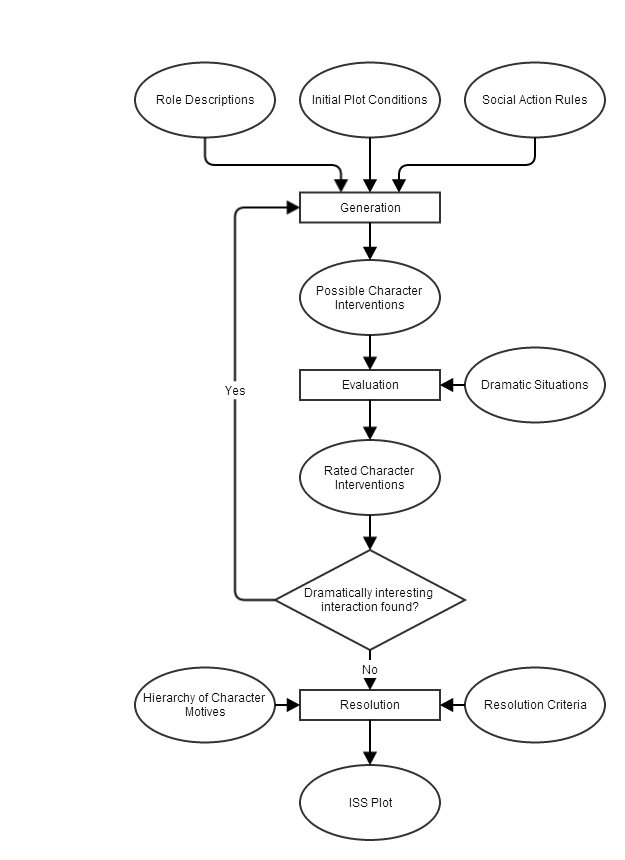
\includegraphics[scale=.6]{sgourosflowchart}
	\caption{Flowchart of Sgouros' \textit{Plot Manager}}
	\label{fig:sgouros_flowchart}
\end{figure}

\section{Character-based storytelling}
At the turn of the century we saw a shift from general story generation towards a more character driven approach.
Researchers like Riedl and Mark\cite{Riedl03character-focusednarrative}\cite{riedl2010narrative} and Marc Cavazza\cite{Cavazza:2002:CIS:630325.630747} wanted to make characters within the story context be more outspoken and distinct and worked towards systems that made this possible.
Most of my work has been based on and influenced by Mark Riedl and Michael Young who contributed to the computational planning of a story.
With their papers\cite{Riedl03character-focusednarrative}\cite{Riedl:2003:MIU:860575.860694}\citep{Riedl:2004:IPM:1018409.1018753} they tackle a multitude of challenges from story planners that use character intent to dealing with interactions between users and agents.
They co-authored the IS system \textit{Mimesis}\citep{young2003towards}, that allows storytellers to use a author-centric approach to generating different stories.
My own planning system (further discussed in chapter~\ref{ch:planning}) has taken a similar route as the systems proposed by Riedl and Young.

\section{Generative narrative within games}
I stated at the beginning of this chapter that most research on the subject of narrative generation takes place within the field of interactive storytelling, but there are some commercial games that have used a form of generative narration.
In \gameby{The Elder Scrolls V: Skyrim}{Bethesda Game Studios} the developers implemented a system they called \textit{Radiant A.I.} that tries to dynamically react to the player's actions.
For example, players with a high \textit{Pickpocket} skill would get told to "keep their hands to themselves" by guards.
The \textit{Radiant Quest} system expands on this, giving players quests that suit their skills and send them to places previously unvisited.
This context is usually used within games; representing a 'fixed' story, but with subtle variance that lets each player have their own experience within a game world.


\section{Conclusions}
The related work done within this field is vast.
So vast perhaps, that to dissect it all greatly exceeds the scope wherein this thesis operates.
But most of the research has been focussed on generating a narrative that is "fixed" from the beginning with some leeway towards actual context.
The usage of a narrative planner is almost universal to ensure any kind of plot coherence, as is a form of author input to control the flow of a story.
These basic elements create a interactive story system that can deliver powerful narratives with believable characters.
My own concern is the involvement of the player.
In most examples the player is merely an actor with a more volatile behaviour, instead of his own character.
I strive for a system that really revolves around the player.
The story made by the actions that the player did or did not do.






\chapter{Narrative planning}
\textit{This chapter will discuss the use of a narrative planner as used by many of my sources. I want to incorporate a narrative planner that smartly uses \diage to manipulate a narrative and conveys that in a way we petty humans can understand}
\\\\
A lot of related work as gone into the use of a planning system that decides on the narrative structure. Researchers like Riedl~\cite{Riedl03character-focusednarrative}\cite{Riedl:2003:MIU:860575.860694}\cite{Riedl:2004:IPM:1018409.1018753} and Cavazza~\cite{Cavazza:2002:CIS:630325.630747} have been researching the use of artificial intelligence for years, and have made some interesting planning systems like \textit{Memesis}~\citationneeded. I am developing my own planning system to use \diage as input and output and use \textit{Ludoscope} to manipulate the diagram as a graph (see section~\ref{sec:ludoscope} for more on Ludoscope) for the model transformations. 
\chapter{Diage Modelling Language}
In this chapter I will cover the Diage Modelling Language (DML) that is used to visualize the flow of information, some are static and others will wait for the interaction of the player to release this information and ensuring plot progression. \diage uses the symbols to represent the \diage entities as seen in figure~\ref{fig:DMLSymbols}. 
\begin{figure}[h]
	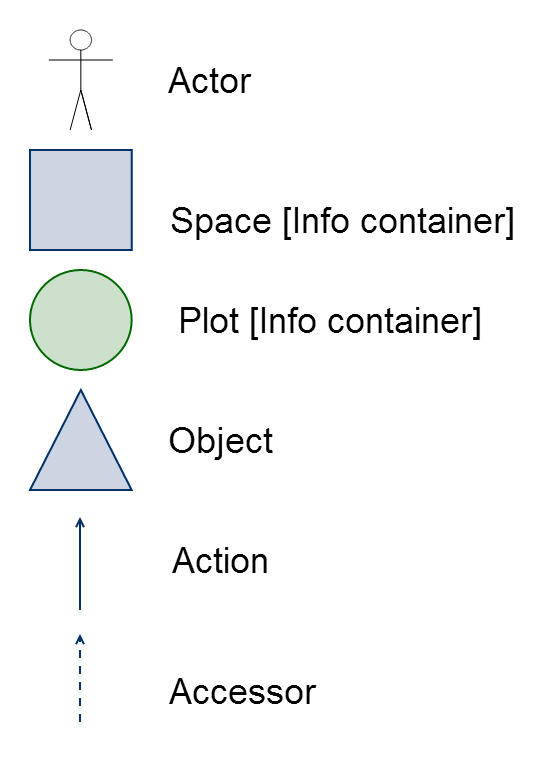
\includegraphics[scale=.3]{symbols}
	\caption{DML Symbols}
	\label{fig:DMLSymbols}	
\end{figure}
\section{Entities}
\diage entities come in four forms; \code{Actors}, \code{Objects}, \code{Spaces} and \code{Events}. The latter two are also information containers which I will discuss in section~\ref{sec:informationcontainers}. The following section will only cover the pure entities; the objects and actors. In conjunction with \code{actions} and \code{accessors} these entities convey story information and plot progression. 
\subsection{Objects}
\diage objects form the basis of all entities. They represent the props and items that we find in the world that have narrative importance. For example; if the Player walks in to a shop \diage does not specify all items that one could buy in the shop, but only those that have plot importance. In terms, these objects should adhere to the \textit{Checkhov's Gun} principle. This dramatic principle states that all objects used in a narrative should eventually be used. I quote: "\textit{One must never place a loaded rifle on the stage if it isn't going to go off. It's wrong to make promises you don't mean to keep.\footnote{\url{http://berlin.wolf.ox.ac.uk/lists/quotations/quotations_by_ib.html}}}"
Objects have three properties; a \code{name}, a \code{ID} and a \code{type} The ID is a unique identifier dependant on the type. And the type is used with actions/accessors as seen in figure~\ref{fig:actions} (Futher discussed in section~\ref{sec:actors}). The name is the noun given to an object within the story context. For example; The player receives the \textit{Skeleton Key of Awesomeness}, but the type is just \code{key} giving it no special properties than any other key. It might make sense to name an object something else than it's type, but a name is not given it defaults to it's type. 
Objects form the world, and all other entities derive from the \diage object. This means that all entities have the same properties as the object, but can extend upon it.
\subsection{Actors}
\label{sec:actors}
An actor is the representation of any one object that can, as the noun implies, act. Examples are the store-clerk, a wandering adventurer or the player. The actor is the only entity that can physically interact with the world, and by doing so the only that can change the world's state. By being able to change the world, the actors are the only entities that can ensure plot progression. 
Just like the object, an actor has three properties; a \code{name}, a \code{ID} and a \code{type}. The type property is used in predefined actions as seen in figure~\ref{fig:actions:npc}. This figure defines that the \code{Player} can \textbf{speak} to all actors of type \code{NPC}. A further glance at figure~\ref{fig:actions} shows some more actions that could be defined for the player actor. These predefined actions tell us that the player can trigger all events and enter all spaces. I will expand upon these actions in section~\ref{sec:actions_and_accessors}.

\section{Information Containers}
\label{sec:informationcontainers}
Information containers are entities that hold story information. A space holds information about it's spacial children, and events release information into spaces when they are resolved. Information containers have the unique property that they are nestable. For example; a space that represents a city can hold several spaces that represents housing. 

\subsection{Spaces}
A space is the representation of any segment of the world or the world itself. As spaces are info containers they are nestable, as mentioned before, but they differ in the fact that they can hold every entity as a child. These children make up the spacial awareness of the space and tells us what information it can pas on to actors. Usually an actor gains all the information a space can give upon the moment it enters the space; when the actor becomes a child object to the space. This can be modified, and some parts of information maybe withheld from the actor, but this is where the events come in.

\subsection{Events}
A event is the odd one out as an entity, as it is the only one that does not represent something within the narrative. A event is the abstraction of information that is released into the story when an actor - usually the player - interacts with it, thus events are used for story pacing and narrative convenience. When we need the state of a space to change we use a event to initiate that change. This only applies on the narrative context of the world, because \diage does not specify everything that happens with in the interactive context. For example; if the player went to a store to buy some cheese to eat. \diage only specifies the store's loss of the cheese, if said food item is a special narrative item. Like a poisonous piece of cheese that the villain left there as a cunning trap for our hero. Events make the world go round and are the dynamic forces in \diage.

\section{Actions and Accessors}
\label{sec:actions_and_accessors}
Actions and accessors are the abstract connectors in \diage. They convey what actors can do (actions) and what knowledge they possess (accessors). Some accessors are implied, due to the fact that an actor might be the child of a space, in other cases these connections are explicitly added to a \diage model. If we review the diagram in figure~\ref{fig:examplediagram} we see that the mayor has no connections whatsoever. This would imply that the Mayor has no knowledge about what's or who's in the store. If we compare that figure to figure~\ref{fig:example:accessors}, we see that the Mayor now has a connection to the Shop, thus we can be sure that the Mayor has the knowledge it would have, if it had been in the shop space itself.

\begin{figure}[ht]
	\centering
	\begin{subfigure}[b]{0.3\textwidth}
		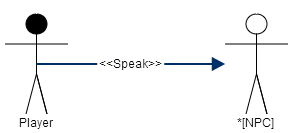
\includegraphics[width=\textwidth]{npc_action}
		\caption{A standard action for NPC interaction}\label{fig:actions:npc}
	\end{subfigure}
	\begin{subfigure}[b]{0.3\textwidth}
		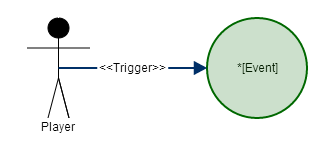
\includegraphics[width=\textwidth]{event_action}
		\caption{A standard action for event interaction}\label{fig:actions:event}
	\end{subfigure}
	\begin{subfigure}[b]{0.3\textwidth}
		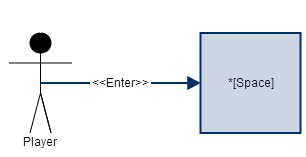
\includegraphics[width=\textwidth]{space_action}
		\caption{A standard action for space interaction}\label{fig:actions:space}
	\end{subfigure}
	\caption{Predefined actions}\label{fig:actions}
\end{figure}

\begin{figure}[ht]
	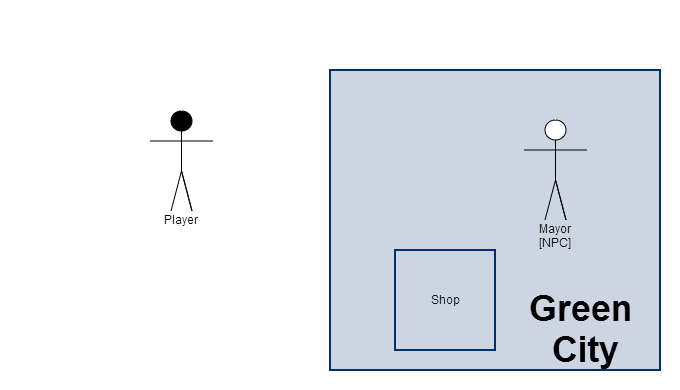
\includegraphics[scale=.5]{diagram_actor_example}
	\caption{An example of a Diage diagram using predefined actions}\label{fig:examplediagram}
\end{figure}
\begin{figure}
	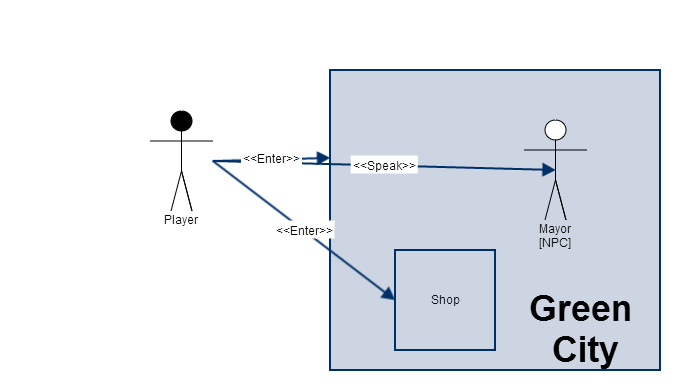
\includegraphics[scale=.5]{diagram_actor_example_verbose}
	\caption{An example of a Diage diagram without using predefined actions}\label{fig:examplediagramverbose}
\end{figure}
\begin{figure}
	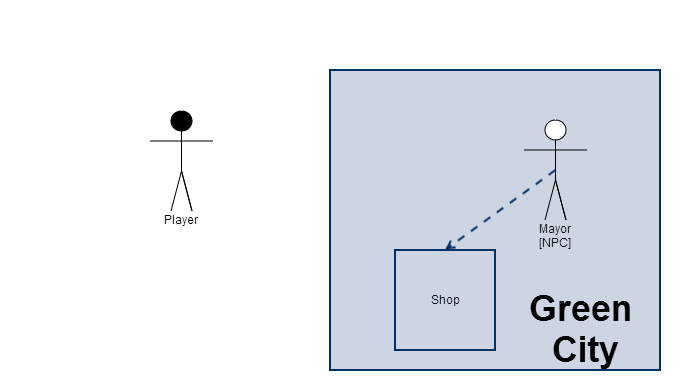
\includegraphics[scale=.5]{diagram_accessor_example}
	\caption{A \diage diagram showing a explicit connection between the Mayor and the Shop}
	\label{fig:example:accessors}
\end{figure}
\section{Diage as a graph}
Diage can be defined by DML, but also as a graph. This form of representation allows us to use graph theory to manipulate and transform the diagram, which we'll cover in the next chapter\footnote{SHOULD BE LEFT FOR FINAL!}

\begin{figure}
	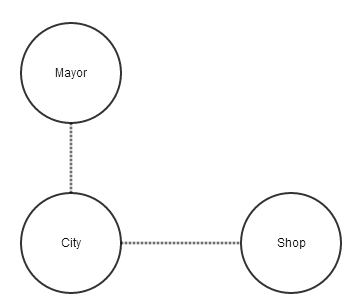
\includegraphics[scale=.5]{diagram_graph}
	\caption{Figure~\ref{fig:examplediagram} as a graph}\label{fig:example:graph}
\end{figure}
\chapter{Rouge}
\begin{quotation}
\textsl{You are a nameless traveller that has been compelled to search for something. An object, a person, or just a place. You don't know yet, but it's up to you to find out. You will travel through various caves, forests and towns to pursue the whims of your heart. Every time you seem to solve a problem, another one turns up. Always moving you towards some inevitable doom. Are you born for heroism, or will you die unloved and unknown? \\\\Choose your path, and see where the voices in your head take you.}
\end{quotation}
Rouge is a \rogue tile-based game that is created specifically for the demonstration of the \diage narrative generation system. Created within my own framework \textit{SilicaLib} created on top of the XNA game-framework created by Microsoft. Rouge is characterised by the fact that the world and the narrative is generated by the direct influence of the player.

\section{Mechanics}
In Rouge, the player moves through the world one tile at a time. 

\section{World generation}
The world within Rouge is procedurally generated by a cellular automaton. During a step of this automaton, the algorithm walks through the game world and checks each tile for certain conditions pertaining to their neighbours. If these conditions are met, his state will be changed accordingly. The states a tile has in Rouge are a simple \textit{alive} or \textit{dead} state. When a tile has 5 or more live neighbours, the tile becomes alive themselves. However, when a tile has less than 2 live neighbours, the tile dies. The first rule ensures that tiles group together, and the other rule destroys any singular 'island' tiles.

\begin{algorithm}
	\KwIn{tilemap}
	\KwOut{new tilemap}
	let \textit{deadCells} and \textit{liveCells} be an empty collection of tiles\;
	\ForEach{tile in tilemap}{
		\uIf{tile.neighbours $\geq$ 5}{
			liveCells.push(tile)\;
		}\uElseIf{tile.neighbours $\leq$ 1}{
			deadCells.push(tile)\;
		}
	}
	\ForEach{tile in deadCells}{
		tile.alive = false\;
	}
	\ForEach{tile in liveCells}{
		tile.alive = true\;
	}
	\caption{Cellular Automation algorithm as used in Rouge}\label{alg:ca}
\end{algorithm}

\begin{figure}
	\centering
	\begin{subfigure}[b]{0.3\textwidth}
		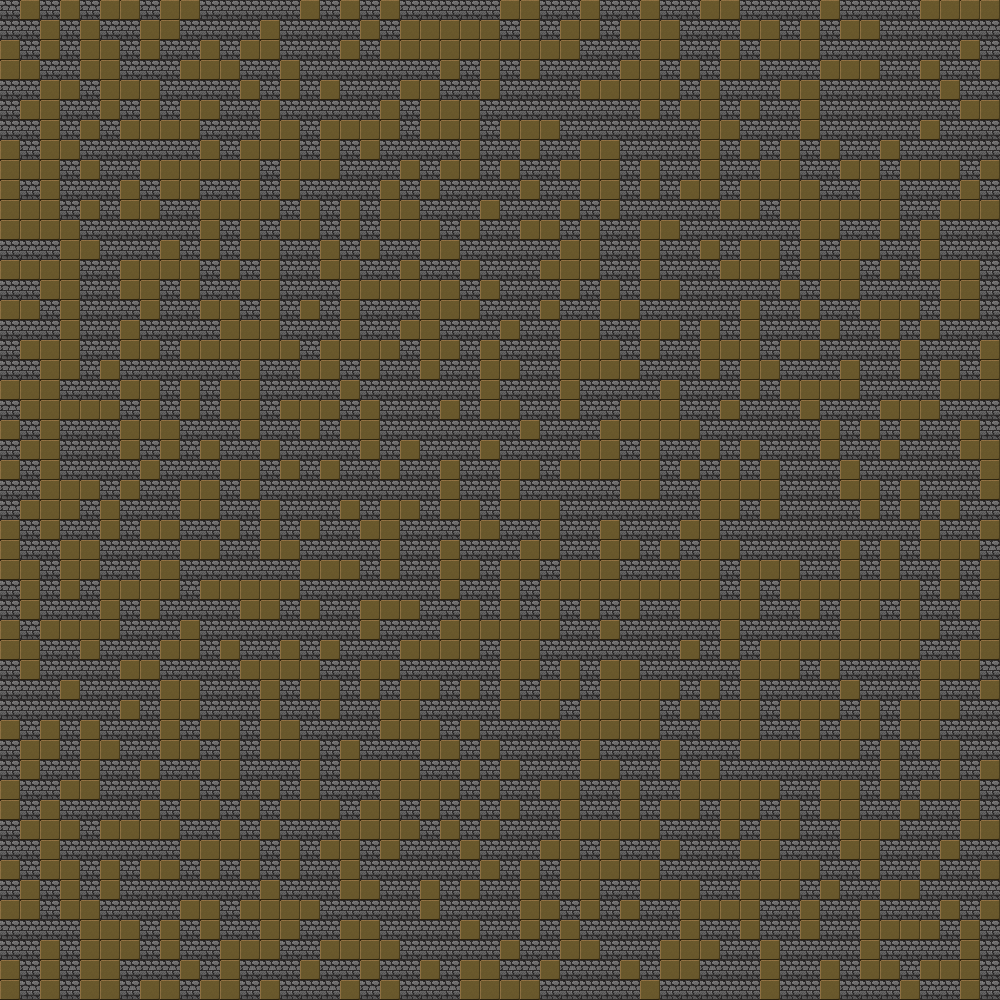
\includegraphics[width=\textwidth]{rouge/screenshot0}
		\caption{Initial map}
	\end{subfigure}	
	~
	\begin{subfigure}[b]{0.3\textwidth}
		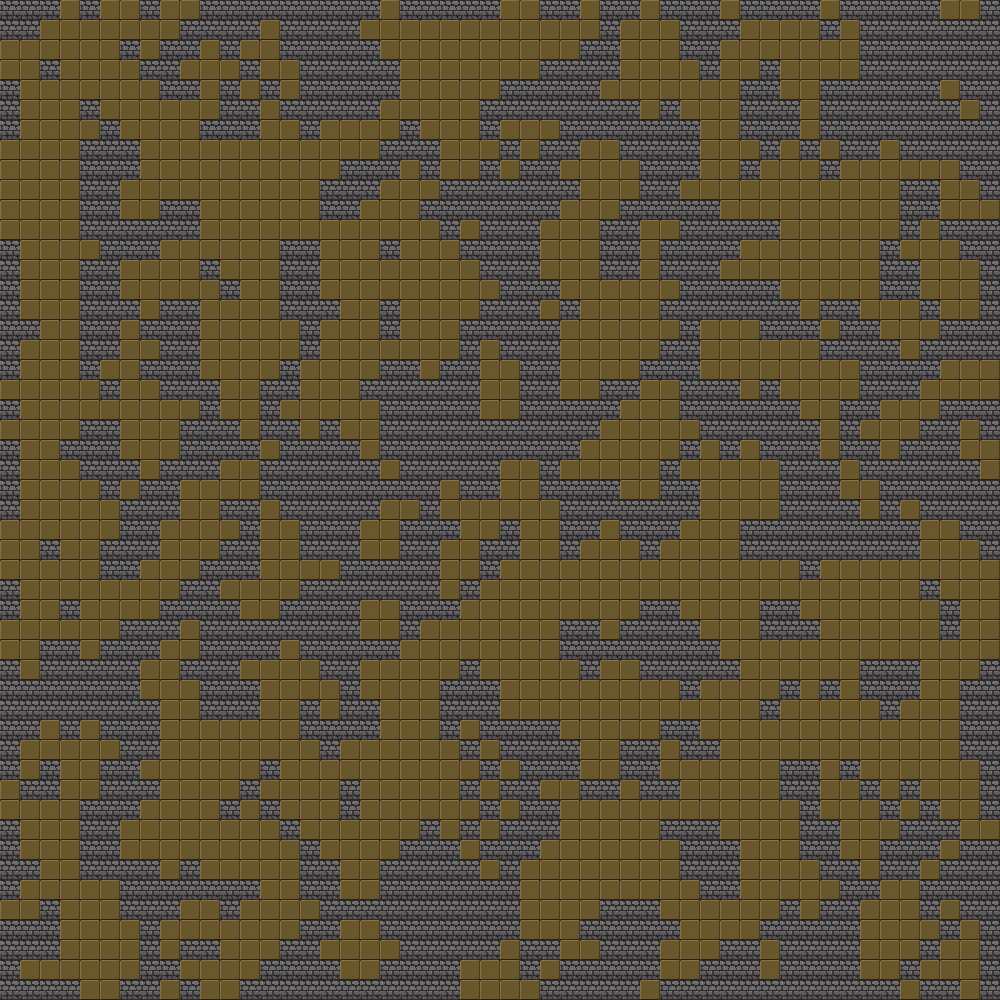
\includegraphics[width=\textwidth]{rouge/screenshot1}
		\caption{Step 1}
	\end{subfigure}	
	~
	\begin{subfigure}[b]{0.3\textwidth}
		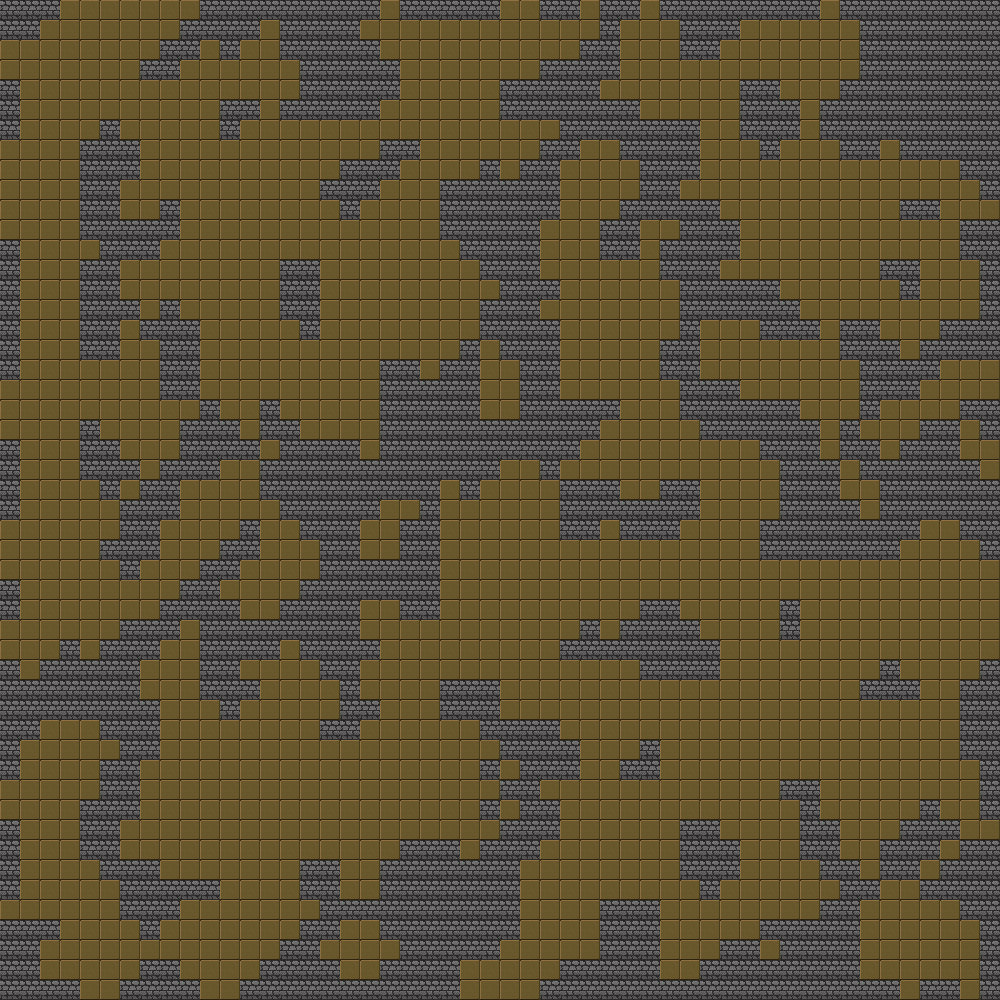
\includegraphics[width=\textwidth]{rouge/screenshot2}
		\caption{Step 2}
	\end{subfigure}	
	~
	\begin{subfigure}[b]{0.3\textwidth}
		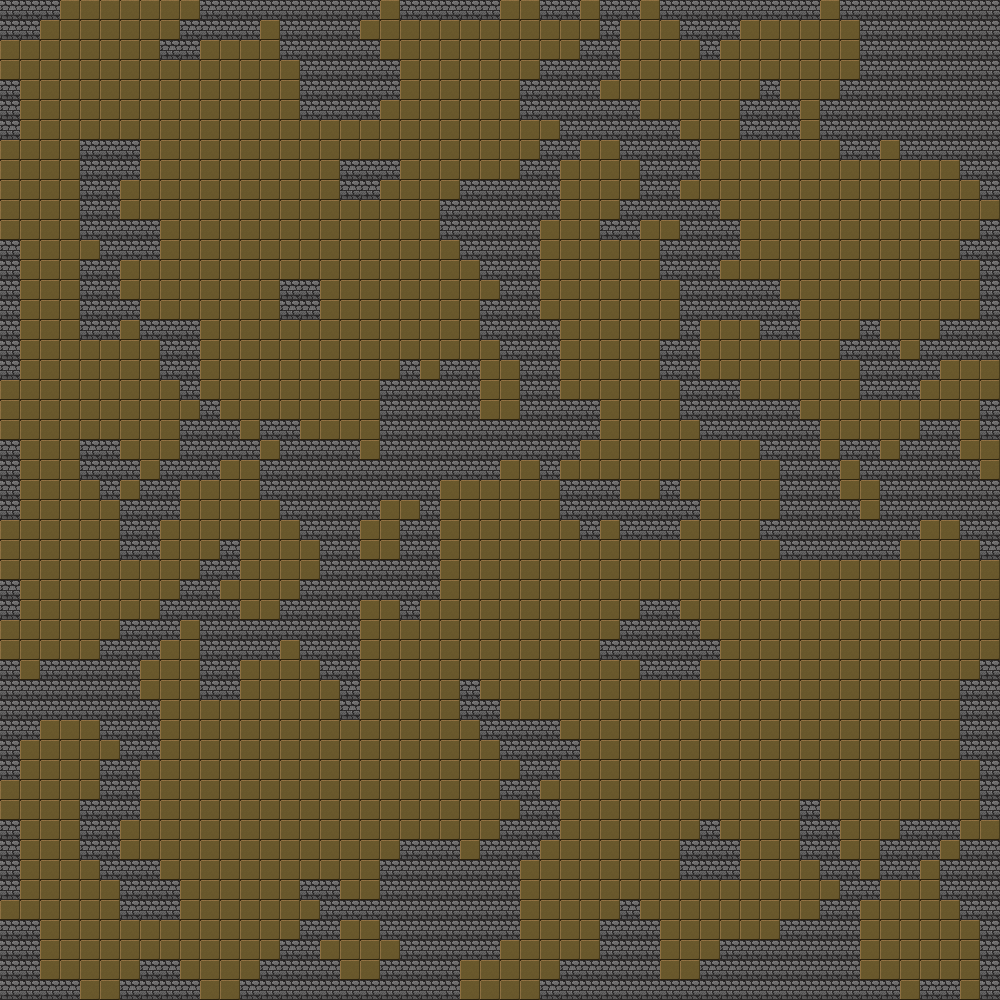
\includegraphics[width=\textwidth]{rouge/screenshot3}
		\caption{Step 3}
	\end{subfigure}		
	~
	\begin{subfigure}[b]{0.3\textwidth}
		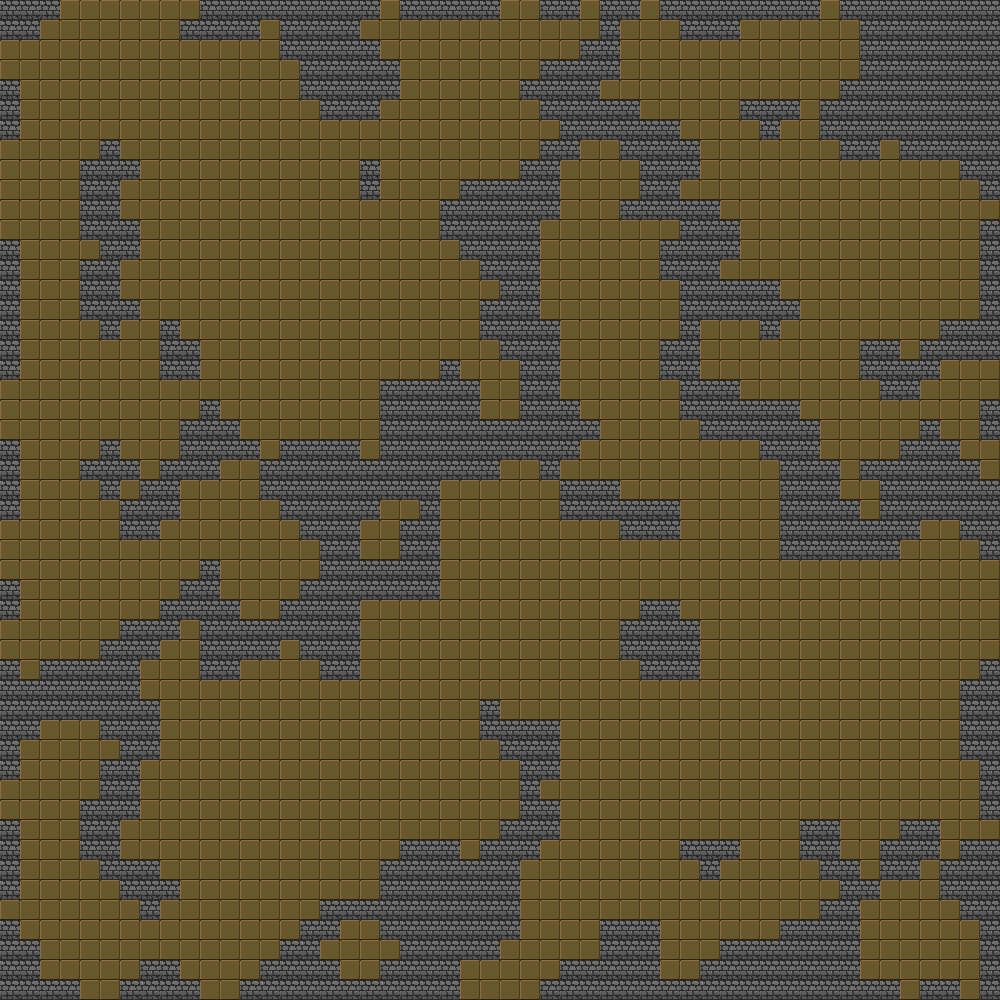
\includegraphics[width=\textwidth]{rouge/screenshot4}
		\caption{Step 4}
	\end{subfigure}
	~
	\begin{subfigure}[b]{0.3\textwidth}
		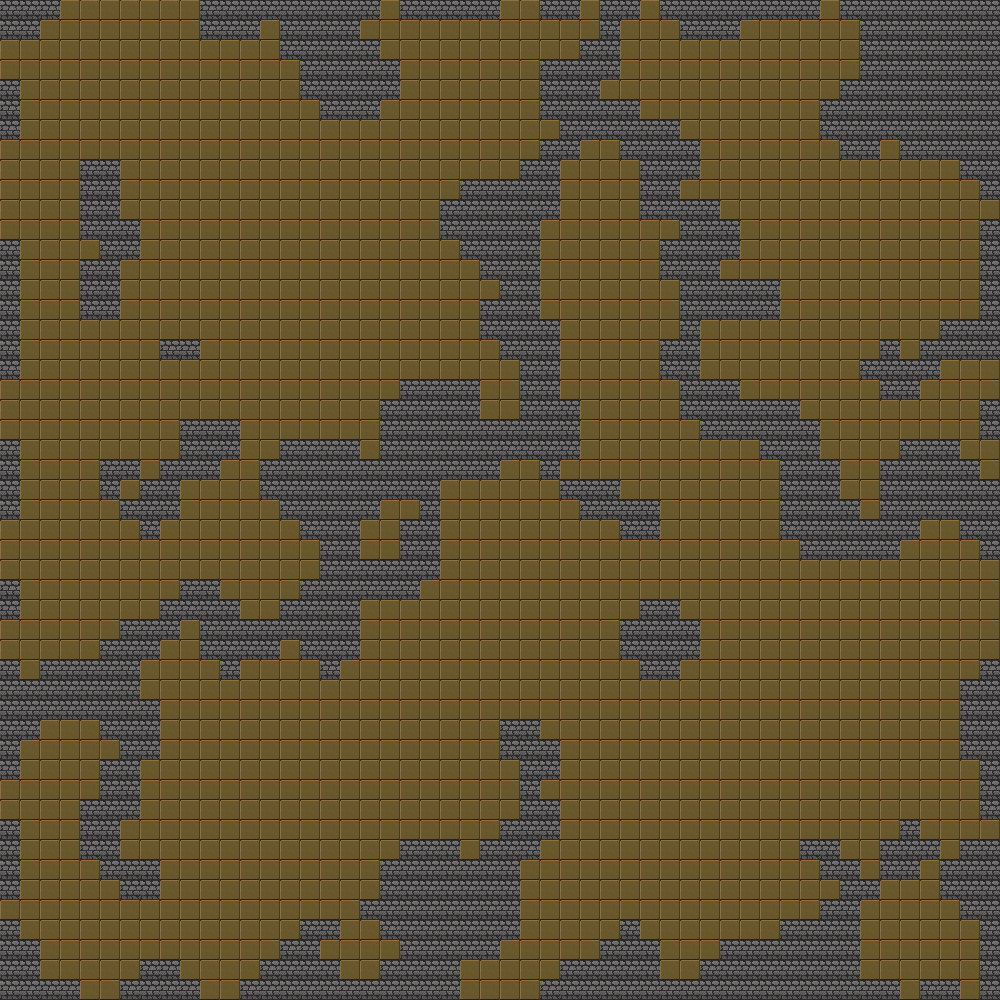
\includegraphics[width=\textwidth]{rouge/screenshot5}
		\caption{Step 5}
	\end{subfigure}	
	\caption{The generation of a 50 x 50 tilemap with 20 x 20 (pixels) tiles}\label{fig:rouge:screens}
\end{figure}
\chapter{Conclusion}
Procedural content is a large part of the \rogue experience. 
In this research, the procedural content is mainly focussed on generating a story, but features world generation as well.
That generation is used to create new scenarios on a fast pace, and requires less time to craft the levels by hand.
Additionally, for the specific case of roguelikes, without novel levels and a new way to traverse the world on every play through, the concept of turn-based dungeon crawling with perma-death quickly loses its appeal.

My goal with procedural narrative planning was to create a rougelike game that creates a controlled narrative in the vain of the rougelike experience: different on every play-through.
I achieved this result by using a narrative planner that combines relationships that in game actors have with other entities - either other actors or objects - and the attributes the actors have to steer the player in a new direction.

To help me create this narrative planner I developed my own modelling language DML (Diage Modelling Language), that served as a visualisation for storytelling.
It uses the entities \textit{spaces}, \textit{actors}, and \textit{objects} to display story states and possible actions that can be taking by the actors to progress onto the next story state. 

I hold that procedural narrative has value within video game development as a whole.
In 20 weeks I've built a system that enables a developer to create games that generate an emergent narrative as a result of simple values given to simple representations.
In chapter~\ref{ch:planning} I reasoned that for my scope and time going forward with a narrative planner was the way to go, in contrast to a BDI system.
A narrative planner gives me much more control over the narrative system, whereas a BDI model would not. 
My conclusion is, however, that any further development of the narrative system should contain a form of the BDI model, with the Narrator as overall director of the actors. 
While true that my research focuses on one type of game, the field is open for further work into other genres.
The Narrator itself can help developers create \rogue games within a smaller time-frame, due to the fact that the Narrator handles most of the story-writing.
Using the Narrator a designer could design a game around the ambiguity of the context, with the inherent fact that every play through can give a player a sense of an actual new adventure.
Even without the use of the Narrator, the attribute system allows designers to design and test any game that has a implicit use of numbers, such as RPGs, Dungeon Crawlers and Tactics games.

As a summary; the development process gets the added benefit of a quick way to prototype stories in the form of the DML diagrams, a fast and efficient way of adding and perfecting game mechanics by the use of the narrative attribute system, and gains the ability to generate unique and novel narratives that is highly controllable, but requires relatively little input.
\chapter*{Reflection}
I feel that a good grasp on agile software development strengthens any developer in his work.
In any team effort I will always try to ensure that all team members have the same idea on how the development process should go, but not so much in any solo project.
I have the impression that my efforts on solo projects are less disciplined than when in a team and as such decided to use a more agile approach in the form of a \textit{design - develop - test - repeat} iterative process to try and structure my own projects.
\subsection*{What went wrong?}
When we started this project, I had no idea of the field I was getting into. 
I had some previous knowledge on the world of Interactive Storytelling, but not to the extent of my own research goals.
As a result, I spend a lot of time reading paper after paper on the idea of generating an interactive story.
With half of the project time spend reading, there wasn't a lot of time left to build and test my theories on how to implement a storytelling algorithm for video games, resulting in me pressing for time to get the product and my thesis done.
To make matters worse, during the last month of the project I decided to take on a completely different tract with my research, throwing away most of the work done already so I could do it properly.
This enormous set-back was the result of figuring out what kind of product I wanted to make, with the consequence that I was just trying a lot of things out and became jumbled.
\subsection*{What went right?}
I've always believed that good software comes from good processes, and this project was a great way to ingrain that in to my way of working. 
Instead of thinking of the product as a whole, I started to focus on what the functionalities where that I needed.
Each functionality was first designed and developed to work alone, and only when this tested positive it was included within the greater whole.
with no concrete idea of what the end result would be, I had no distractions as to work towards an actual product.
We had a feature-set that stated what we wanted to accomplish, and that was my guidance for the project.
\subsection*{Conclusion}
This method of working really suited me and helped me focus on the task at hand, without losing sight of the bigger picture.
I am of the opinion that software development could benefit a lot with this form of looking at a product.
Developers of a product can have a general idea for what the end result could be, but the spotlight should be on the requirements at hand, and solving them one by one until a product comes out of it. 
\bibliographystyle{plain}
\bibliography{diage}
\end{document}